\makeheading{2019-10-24}
\begin{thmbox}
    \begin{theorem}[Fundamental Theorem of LP]
        Let (P) be an LP problem. Then exactly one of the following holds:
        \begin{itemize}
            \item (P) is infeasible
            \item (P) is unbounded
            \item (P) has an optimal solution
        \end{itemize}
    \end{theorem}
\end{thmbox}
\begin{remark}
    Fundamental Theorem of LP and Fundamental Theorem of LP (SEF) are not
    the same, they are two completely different theorems!
\end{remark}

\section{Geometry}
\subsection{Feasible Region of LPs and Polyhedra}

\begin{defbox}
    \begin{definition}
        Let $ \bm{a} \in \mathbb{R}^n\setminus{\bm{0}} $, $ \beta \in\mathbb{R} $.

        $ H:=\left\{\bm{x}\in\mathbb{R}^n:
            \bm{a} ^\top \bm{x}=\beta \right\} $ is a \emph{hyperplane}.

        $ F:=\left\{\bm{x}\in\mathbb{R}^n:
            \bm{a} ^\top \bm{x}\leqslant \beta\right\} $ is a \emph{half-space}.
    \end{definition}
\end{defbox}

Solution sets of linear equations are intersections of hyperplanes.

\begin{defbox}
    \begin{definition}
        Let $ A\in \mathbb{R}^{m \times n} $, $ \bm{b}\in \mathbb{R}^m $.
        $ P:=\left\{\bm{x}\in\mathbb{R}^n:A\bm{x}\leqslant \bm{b}\right\} $ is a \emph{polyhedron}.
    \end{definition}
\end{defbox}
\begin{remark}
    The set of solutions to any one of the inequalities of
    $ A\bm{x}\leqslant \bm{b} $ is a half-space.
\end{remark}

\begin{thmbox}
    \begin{theorem}
        The feasible region of an LP is a polyhedron or equivalently the
        intersection of a finite number of half-spaces.
    \end{theorem}
\end{thmbox}
\begin{proof}
    Let $ \bm{a}\in\mathbb{R}^n,\bm{x}\in\mathbb{R}^n,\beta\in \mathbb{R} $.

    Given an inequality of the form $ \bm{a} ^\top \bm{x}\geqslant  \beta $, we can
    rewrite it as $ -\bm{a} ^\top \bm{x}\leqslant -\beta $.

    Given an equation of the form $ \bm{a} ^\top \bm{x}=\beta $ we can rewrite it as
    $ \bm{a} ^\top \bm{x}\geqslant  \beta $ and $ -\bm{a} ^\top \bm{x}\leqslant -\beta $.

    Thus, any set of linear constraints can be rewritten as
    $ A\bm{x}\leqslant \bm{b} $ for some $ A\in \mathbb{R}^{m \times n} $ and $ \bm{b}\in \mathbb{R}^m $, where $ \bm{a}^\top $ can correspond to each row of $ A $,
    and $ \beta $ can correspond to each row of the column vector $ \bm{b} $.
\end{proof}

Solutions sets of $ A\bm{x}=\bm{b} $ are either $ \emptyset $, a single
point, a line, or in general, an intersection of a hyperplane.

Note that already in $ \mathbb{R}^2 $ there are already equivalent polyhedra.
The mathematical modelling power of LPs are significantly more than that of
linear systems of equations.

\subsection{Convexity}

\begin{defbox}
    \begin{definition}
        The \emph{line segment} joining two points, $ x^{(1)} $ and $ x^{(2)} $ is
        \[ \left\{\lambda x^{(1)} + (1-\lambda)x^{(2)}:\lambda\in[0,1]\right\} \]
    \end{definition}
\end{defbox}
Graphically, the line segment can be seen as:
\begin{center}
    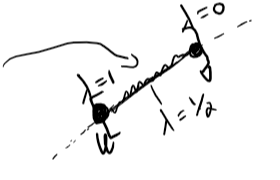
\includegraphics{linesegment}
\end{center}

\begin{defbox}
    \begin{definition}
        A subset $ S\subseteq \mathbb{R}^n $ is \emph{convex} if for
        every pair of points $ x^{(1)},x^{(2)}\in S $, the line segment with
        ends $ x^{(1)} $ and $ x^{(2)} $ is included in $ S $. That is,
        \[ \left\{\lambda x^{(1)} + (1-\lambda)x^{(2)}:\lambda\in[0,1]\right\}\subseteq S \]
    \end{definition}
\end{defbox}
\begin{center}
    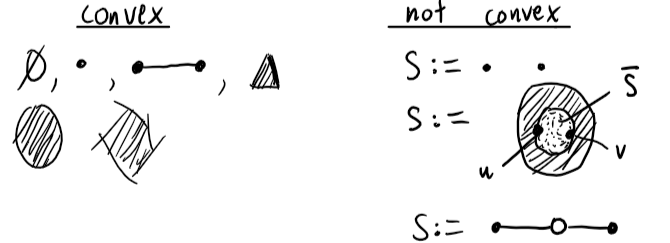
\includegraphics{convex}
\end{center}

\begin{thmbox}
    \begin{theorem}
        Half-spaces are convex.
    \end{theorem}
\end{thmbox}
\begin{proof}
    Let $ H\subseteq\mathbb{R}^n $ be a half-space. Then $ \bm{a} \in \mathbb{R}
        ^n\setminus{\bm{0}} $ and $ \beta\in\mathbb{R}^n $ such that
    \[ H=\left\{\bm{x}\in\mathbb{R}^n: \bm{a} ^\top \bm{x}\le\beta \right\} \]
    Let $ \bar{x}=\lambda x^{(1)} + (1-\lambda)x^{(2)} $ where $ \lambda\in[0,1] $.
    \[ \bm{a}^\top\bar{x}=\bm{a}^\top\left[\lambda x^{(1)} + (1-\lambda)x^{(2)}\right]=
        \underbrace{\lambda}_{\geqslant  0}\underbrace{\bm{a} ^\top x^{(1)}}_{\leqslant \beta}+
        \underbrace{(1-\lambda)}_{\geqslant  0}\underbrace{\bm{a} ^\top x^{(2)}}_{\leqslant \beta}
        \leqslant \lambda \beta + (1-\lambda)\beta=\beta \]
    Thus, $ H $ is convex since $ \bar{x}\in H $.
\end{proof}

\begin{thmbox}
    \begin{theorem}
        The intersection of any collection of convex sets is convex.
        That is, a convex set $ C_j $ for all $ j\in J $, the intersection
        \[ C:=\bigcap_{j\in J} C_j \]
        is convex.
    \end{theorem}
\end{thmbox}

\begin{proof}
    Let $ u,v $ be two points in $ C $. Let $ w $ lie on the line
    segment between $ u $ and $ v $. Then, $ w\in C_j $ since $ C_j $ is convex
    for each $ j\in J $. Thus, $ w\in C $.
\end{proof}

\begin{remark}
    $ J $ can be infinite. That is, the intersection of infinitely many convex sets
    is convex, which can be formally proved by strong induction.
\end{remark}

\begin{thmbox}
    \begin{theorem}
        Polyhedra are convex.
    \end{theorem}
\end{thmbox}

\begin{defbox}
    \begin{definition}
        We say that a point $x$ is \emph{properly contained} in a line segment if it is in the line segment
        and not an endpoint.
    \end{definition}
\end{defbox}

\subsection{Extreme Points}

\begin{defbox}
    \begin{definition}
        Let $ S\subseteq \mathbb{R}^n $ be a convex set.
        Let $ \bar{x}\in\mathbb{R}^n $.
        $ \bar{x} $ is an \emph{extreme point} of $ S $, if $ \bar{x}\in S $ and
        no line segment that properly contains $ \bar{x} $ is included
        in $ S $.

        Equivalently, $ \bar{x} $ is an \emph{extreme point} of $ S $, if
        $ \bar{x}\in S $ and no two distinct $ x^{(1)},x^{(2)}\in S $ exist satisfying
        \[ \bar{x}=\lambda x^{(1)} + (1-\lambda)x^{(2)} \]
        for some $ \lambda\in (0,1) $.

        Equivalently, $ \bar{x} $ is an \emph{extreme point} of $ S $, if
        $ \bar{x}\in S $ and no two distinct $ x^{(1)},x^{(2)}\in S $ exist satisfying
        \[ \bar{x}=\frac{1}{2} x^{(1)} + \frac{1}{2} x^{(2)} \]
    \end{definition}
\end{defbox}

\begin{center}
    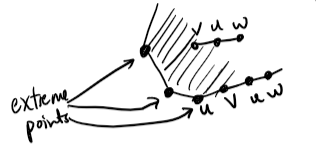
\includegraphics{extremepoint}
\end{center}
